\documentclass{article}

\usepackage{tikz}

\def\prob{\prod_{1 \leq j \leq k \leq n} a_j a_k}

\title{Concrete Math Ch 2 Problem 26}
\author{Daniel Werner}

\begin{document}

\maketitle

\section*{Problem Statement}

Write the following double product as a single product:

\begin{equation}
    P = \prob
\end{equation}

\section*{Solution}

\def\jkunordered{\prod_{1 \leq j, k \leq n} a_j a_k}
\def\konly{}

The terms in this double product can be thought of as
    taking place on a grid of terms depicting each possible
    two-tuple of the given index variables given the
    constraints in the subscripts.
    The grid of relevant terms can be depicted as follows:

\begin{center}
    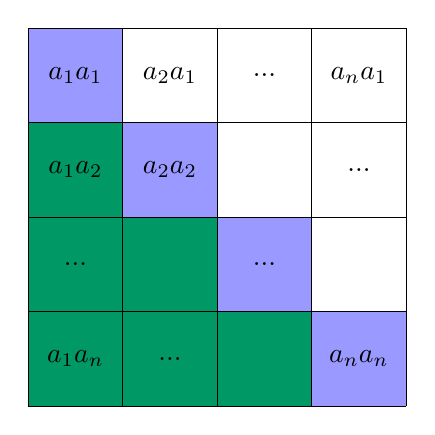
\begin{tikzpicture}
        \fill[blue!40!white] (0,4.8) rectangle (1.2,6);
        \fill[blue!40!green] (0,4.8) rectangle (1.2,1.2);
        \fill[blue!40!white] (1.2,3.6) rectangle (2.4,4.8);
        \fill[blue!40!green] (1.2,3.6) rectangle (2.4,1.2);
        \fill[blue!40!white] (2.4,2.4) rectangle (3.6,3.6);
        \fill[blue!40!green] (2.4,2.4) rectangle (3.6,1.2);
        \fill[blue!40!white] (3.6,1.2) rectangle (4.8,2.4);
        \draw[step=1.2cm,color=black] (0,1.2) grid (4.8,6);
        \node at (0.6,5.4) {$a_1 a_1$};
        \node at (1.8,5.4) {$a_2 a_1$};
        \node at (3.0,5.4) {...};
        \node at (4.2,5.4) {$a_n a_1$};
        \node at (4.2,4.2) {...};
        \node at (0.6,4.2) {$a_1 a_2$};
        \node at (0.6,3.0) {...};
        \node at (0.6,1.8) {$a_1 a_n$};
        \node at (1.8,1.8) {...};
        \node at (1.8,4.2) {$a_2 a_2$};
        \node at (3.0,3.0) {...};
        \node at (4.2,1.8) {$a_n a_n$};
    \end{tikzpicture}
\end{center}

With this diagram, the relevant sub-products can be identified.
The diagonal, in blue where the indices are all the pairs
of equal value, is easiest:

\begin{equation}
    diagonal = \prod_{1 \leq j = k \leq n} a_j a_k = 
    \prod_{1 \leq k \leq n} a_k^2 =
    \left( \prod_{1 \leq k \leq n} a_k \right)^2
\end{equation}

The diagonal is easy to reduce to a single index variable.
The product in the problem however represents all of the
colored squares on the diagram, i.e. the index combinations
where the j values are less than or equal to the k values.

\par

It is worth noting that the symmetry of the square would
indicate that a product consisting of the colored squares flipped
along the diagonal would be equal.  This process would represent
simply renaming or swapping the index variables.

\par

The green triangle is just the product of all the terms where
$j < k$, so:

\begin{equation}
    triangle = \prod_{1 \leq j < k \leq n} a_j a_k
\end{equation}

Given the symmetry of the green triangle rotating about the
diagonal and combined with the diagonal itself, we can
observe that:



\begin{equation}
    wholegrid = triangle^2 \cdot diagonal
    = \left( \prod_{1 \leq j < k \leq n} a_j a_k \right)^2
    \cdot \left( \prod_{1 \leq k \leq n} a_k \right)^2
\end{equation}

Another expression for the whole grid is:

\begin{equation}
    wholegrid = \prod_{1 \leq j, k \leq n} a_j a_k 
    = \left( \prod_{1 \leq j \leq n} a_j \right)^n
    \cdot \left( \prod_{1 \leq k \leq n} a_k \right)^n
    = \left( \prod_{1 \leq k \leq n} a_k \right)^{2n}
\end{equation}

Meaning that

\begin{equation}
    wholegrid = \left( \prod_{1 \leq k \leq n} a_k \right)^{2n}
    = \left( \prod_{1 \leq j < k \leq n} a_j a_k \right)^2
    \cdot \left( \prod_{1 \leq k \leq n} a_k \right)^2
\end{equation}

\begin{equation}
    \left( \prod_{1 \leq k \leq n} a_k \right)^n
    = \left( \prod_{1 \leq j < k \leq n} a_j a_k \right)
    \cdot \left( \prod_{1 \leq k \leq n} a_k \right)
\end{equation}

\begin{equation}
    triangle = \left( \prod_{1 \leq j < k \leq n} a_j a_k \right)
    = \frac{\left( \prod_{1 \leq k \leq n} a_k \right)^n}{\left( \prod_{1 \leq k \leq n} a_k \right)}
    = \left( \prod_{1 \leq k \leq n} a_k \right)^{n - 1}
\end{equation}

Now that we have two single-index expressions for the
components of $\prob$, we can just combine:

\begin{equation}
    \prob = triangle \cdot diagonal
    = \left( \prod_{1 \leq k \leq n} a_k \right)^{n - 1}
    \cdot \left( \prod_{1 \leq k \leq n} a_k \right)^2
\end{equation}

\begin{equation}
    P = \prob = \left( \prod_{1 \leq k \leq n} a_k \right)^{n + 1}
\end{equation}

\end{document}